\documentclass[../em.tex]{subfiles}
\graphicspath{{\subfix{../figures/}}}
\begin{document}
\chapter{Electric Charges, Fields and Gauss's Law}
\section*{Brief Calculus Review}
The derivative of a function at some point characterizes the rate of change of the function at that point; 
The rate of change of the function is basically the slope at that point.

Because the derivative is a slope, the notation can be written as 
\[f'(x)=\frac{\mathrm{d}x}{\mathrm{d}t}\]

There are some derivative rules to know.
\begin{itemize}
    \item $\frac{\mathrm{d}}{\mathrm{d}x} = 0$
    \item $\frac{\mathrm{d}}{\mathrm{d}x}(x) = C$
    \item $\frac{\mathrm{d}}{\mathrm{d}x}x^n = nx^{n-1}$
    \item $\frac{\mathrm{d}}{\mathrm{d}x}(f(x)\pm g(x))=\frac{\mathrm{d}}{\mathrm{d}x}f(x)\pm \frac{\mathrm{d}}{\mathrm{d}x}g(x)$
\end{itemize}

An integral is simply finding the area under a curve. 

The integral notation is:
\[f(x)=\int{f'(x)\mathrm{d}x}\]

In physics, we use the definite integral, where the area is found over an interval $[a,b]$.

The notation for this is:
\[A = \int_b^a{f'(x)\mathrm{d}x}=f(b)-f(a)\]

There are some integration rules to know as well.
\begin{itemize}
    \item $\int{\mathrm{d}x} = x+C$
    \item $\int{x^n\mathrm{d}x}=\frac{1}{n+1}x^{n+1}, n \neq -1$
    \item $\int{f(x)\pm g(x)\mathrm{d}x}=\int{f(x)\mathrm{d}x}\pm \int{g(x)\mathrm{d}x}$
\end{itemize}

A differential equation is an equation involving one or more derivatives of an unknown function. 
The order of a differential equation is defined to be the order of the highest derivative it contains.

All differential equations are considered to be separable and can be solved by integration. This process is called separation of parts.

Much like derivatives there are set of integrals that don't follow the basic power rule of integration. There are some special integral rules.
\begin{itemize}
    \item $\int{e^{ax}}\mathrm{d}x=\frac{1}{a}e^{ax}+C$
    \item $\int \frac{\mathrm{d}x}{x+n}=\ln |x+a|+C$
    \item $\int \cos(ax)\mathrm{d}x = \frac{1}{a}\sin(ax)$
    \item $\int \sin(ax)\mathrm{d}x=-\frac{1}{a}\cos(ax)$
\end{itemize}

Integration by substitution is a way of undoing the derivative's chain rule. You need the integral to look like this:
\[\int f(g(x))g'(x)\mathrm{d}x=\int f(u)\mathrm{d}u\]

Here are some special derivatives:
\begin{itemize}
    \item $\frac{\mathrm{d}}{\mathrm{d}x}e^{ax}=ae^{ax}$
    \item $\frac{\mathrm{d}}{\mathrm{d}x}\ln ax = \frac{1}{x}$
    \item $\frac{\mathrm{d}}{\mathrm{d}x}\sin ax = a\cos ax$
    \item $\frac{\mathrm{d}}{\mathrm{d}x}\cos ax = -a\sin ax$
\end{itemize}

All derivatives on the formula sheet are written using the chain rule.

The chain rule follows this general rule: 
\[f(g(x))=f'(g(x))\cdot g'(x)\]

A vector is a quantity that has both magnitude and direction. The length of the line shows its 
magnitude and the arrowhead points in the direction.
To add vectors, place the tip of the first vector to the tail of the second vector.
The resultant is the arrow drawn from the tail of the first vector to the tip of the second vector.

The goal of subtracting vectors is to turn it into addition by finding the inverse of the second vector. Basically: 
\[\vec{A}-\vec{B}=\vec{A}+(-\vec{B})\]

When adding or subtracting vectors algebraically, the first thing you need to do is to resolve the vectors into components.
\begin{itemize}
    \item $A_x = A\cos \theta$
    \item $A_y = A\sin \theta$
\end{itemize}

Once all the vectors are broken down, you can add the horizontal and vertical components. 
This will give you the horizontal and vertical components of the resultant.

To find the magnitude of the resultant, you can find the hypotenuse: 
\[R = \sqrt{R_x^2+R_y^2}\]. 

The direction can be found from:
\[\theta = \tan^{-1}\left(\frac{R_y}{R_x}\right)\]

There are times when you need to "scale" up or down a vector. To do so, 
you multiply the magnitude of a vector, but not the direction, by a scalar.

A unit vector has a magnitude of 1 and a direction that goes along one of the axes. 

The dot product is the process of multiplying two vectors and getting a scalar answer in return. There are two ways to find this:
\begin{itemize}
    \item $\vec{a}\cdot \vec{b} = a_xb_x+a_yb_y$
    \item $\vec{a}\cdot \vec{b} = |a||b|\cos \theta$
\end{itemize}

The second method also helps determine if the vectors are orthogonal, or perpendicular to each other.

The cross product is the process of multiplying two vectors and getting a vector in return. 
The answer is a vector that is at a right angle to the two original vectors. The magnitude 
of the cross product equals the area of the parallelogram with the two original vectors as sides.

The cross product is zero in length when the original vectors point in the same or 
opposite directions. It reaches maximum length when the original vectors are at right angles to each other.

There are two ways to calculate the cross product.

The first is:
\[\vec{a} \text{x} \vec{b} = [|a||b|\sin \theta]\hat{n}\]

This method does not give you the direction of the vector.

The second way is to use a set of formulas to find the components:
\begin{itemize}
    \item $C_x=a_yb_2-a_2b_y$
    \item $C_y=a_2b_x-a_xb_2$
    \item $C_z=a_xb_y-a_yb_x$
\end{itemize}

The direction is determined by the right hand rule. Your index finger points in the direction of 
vector $a$, your middle points in the direction of $b$, and your thumb points in the direction of the answer.

\section{Electric Charge and Electric Force}
Electric charge is a fundamental property of all matter.

Charge is scalar value, which means it has no direction, and is described as either positive or negative.

The magnitude of charge on a single electron is the elementary charge which is 
$e = 1.6\times 10^{-19}$ C (coulomb). The coulomb is the unit of charge.

Coulomb's Law describes the electrostatic force between two charges objects. The equation for this is:
\[F_E=\frac{kq_1q_2}{r^2}\]

This equation is similar to the universal gravitation formula. Note that 
$r$ can be written sometimes as $d$, it is the distance between the centers. 
$k$ is the electrostatic constant and is equal to $9\times10^9$N$\cdot $m$^2$/C$^2$. $k$ 
is sometimes written as $\frac{1}{4\pi\epsilon_0}$.

The direction of the electrostatic force depends on the signs. 
Opposite charges attract and like charges repel. Electrostatic force can also cause 
other forces like tension, friction, and normal force.

Electrostatic force can be attractive (different signs) or repulsive (same signs), 
while gravitational force, which is similar, can only be attractive. 

The electrostatic force has a much larger magnitude than gravitational force, but 
gravitational force acts on a larger scale in that the electrostatic force works at a 
microscropic scale, while gravitational force will be on a planetary scale.

Free space (a region where there is no electromagnetic or gravitational fields) has a 
constant value of electric (or vacuum) permittivity which is equal to $\epsilon_0 = 8.85\times10^{-12}$C$^2$/(N$\cdot$m$^2$).

\pagebreak
\begin{example}
    Point charges Q$_1$ = 2.0$\mu$C and Q$_2$ = -4.0$\mu$C are located at $\vec{\text{r}_1} = (4.0\hat{i}-2.0\hat{j}+5.0\hat{k})$m and 
    $\vec{\text{r}_2} = (8.0\hat{i}+5.0\hat{j}-9.0\hat{k})$m. What is the force of Q$_2$ on Q$_1$?

    We have the equation 
    \[F_E=\frac{kq_1q_2}{r^2}\]
    We first have to find the distance between the charges. We can use the distance formula for this:
    \begin{align*}
        r = \sqrt{(x_2-x_1)^2+(y_2-y_1)^2+(z_2-z^1)^2}\\
        r = \sqrt{(8-4)^2+(5+2)^2+(-9-5)^2}\\
        r = 16.2 \text{m}
    \end{align*}

    Now we can plug this into the equation.
    \begin{align*}
        F_E=\frac{kq_1q_2}{r^2}\\
        F_E=\frac{(9\times10^9)(2\times10^{-6})(-4\times10^{-6})}{(16.2)^2}\\
        F_E=-2.74\times10^{-4}\text{N}
    \end{align*}

    Note that since both point charges have opposite signs, they will try and attract each other, which means the resulting force calculated 
    will be negative.
\end{example}

\ex Two small spheres have charges of $2Q$ and $3Q$. When their centers are separated by a distance $d$, they exert an electrostatic force of magnitude $F_0$ on each other. What is the magnitude of the force exerted on two other spheres that have charges of $2Q$ and $9Q$ when their centers are a distance $2d$ apart? 

\ex Two point charges, both with charge $Q$, exert an electrostatic force of magnitude $F_0$ on each other when they are a distance $d$ apart. What is the magnitude of the electrostatic force on two other point charges, each with a charge $2Q$, that are a distance $\frac{d}{3}$ apart?

\section{Conservation of Electric Charge and the Process of Charging}
The net charge or charge distribution of a system can change in response to the prescence of, 
or changes in, the net charge or charge distribution of other systems. For example, the net charge 
can change due to friction or contact between systems.

Induced charge separation occurs when electrostatic force between two systems 
alters the distribution or charges within the systems, resulting in the polarization of 
one or both systems. Induced charge separation can only occur in neutral systems.

Any change to a system's net charge is due to a transfer of charge between the 
system and its surroundings. Most of the time, this is the result of a transfer of electrons.

An application of this is grounding, which involves electricially connecting 
a charged object to a much larger and approximately neutral system (such as the Earth).

\pagebreak
\begin{example}
    There are two identical metal spheres on insulating stands. Sphere 1 has a charge of $-1.02 \times 10^{-16}$C. 
    Sphere 2 has a deficit of 841 electrons. The two spheres are brought together so that they touch each other. 
    They are then separated again so that they are no longer touching. What charge does each sphere have after 
    they have touched? Consider the new charge on Sphere 2. Does this correspond to a deficit or an excess of 
    electrons? How many electrons is the deficit/excess?

    First, we must find the charge on Sphere 2. Because the problem states that there is a deficit of electrons, the charge is positive.
    
    The charge on Sphere 2 is:
    \[841 \times (1.6\times 10^{-19}) = 1.35\times 10^{-16}\text{C}\]

    Now we find the net charge on the system by adding it to the charge on Sphere 1:
    \[1.35 \times 10^{-16} + (-1.02 \times 10^{-16}) = 3.3\times 10^{-17}\text{C}\]

    Now we simply divide this number by two since the charge is divded evenly between the two spheres:
    \[\frac{3.3\times 10^{-17}\text{C}}{2}=1.6\times 10^{-17}\text{C}\]
    
    This answers the first part of the question.

    The new charge is positive, which means there is an deficit of electrons. 
    To find the amount of electrons in this deficit we must convert to electrons:
    \[1.65\times10^{-17}\text{C}\times \frac{1e}{1.6\times10^{-19}\text{C}}=103\text{ electrons}\]
\end{example}

\ex A student has a positively charged insulating cube and a neutral conducting sphere. The student can experiment by performing any of the following actions.
\begin{enumerate}
    \item Touch the cube to the sphere.
    \item Bring the cube near, but not touching the sphere.
    \item Move the cube away from the sphere.
    \item Connect the sphere to the ground.
    \item Disconnect the sphere from ground.
\end{enumerate}
Which actions, and in what order, could the student perform so that the sphere becomes negatively charged?

\ex Two identical conducting spheres have different charges. One sphere has a charge of $+1$ nC, and the other sphere has a charge of $-3$ nC. 
The two spheres are brought into contact and then separated. What is the magnitude of charge that is transferred between the spheres? 
Write an accurate description of how to calculate the magnitude of the transferred charge.

\ex A positively charged glass rod if brought near but does not touch a metal sphere. 
A wire is then used to ground the sphere while the charged rod remains close to it. The grounding wire is disconnected and then the charged 
rod is moved away from the sphere. What is the final net charge on the sphere and provide an explanation.

\pagebreak
\section{Electric Fields}
Electric fields may originate from charged particles.

The electric field at a given point is the ratio of the electric force exerted on a test 
charge at the point to the charge and the charge on the test charge itself.

Mathematically this is:
\[E = \frac{F_E}{q}[N/C]\]

Another way of writing this is:
\[F_E=qE\]

The E-field points away from an isolated positive charge towards an 
isolated negative charge. Therefore, if the test charge is negative, 
the electric force points opposite the direction of the electric field.

\begin{example}
(a) Find the direction and magnitude of an electric field that exerts a $4.80\times10^{-17}$ N westward force on an electron. 

(b) What magnitude and direction force does this field exert on a proton?

For part (a), we use the formula:
\[E=\frac{F_E}{q}=\frac{4.80\times10^{-17}\text{ N}}{1.6\times10^{-19}\text{ C}}=300  \text{ N/C East}\]

For part (b), the proton and electron have the same charge, so they experience the same electric field. 
The force and the E-field because of the positive charge results in the force pointing in the same direction, so 300 N/C West.
\end{example}

\ex Two spheres having charges of $+3Q$ and $-Q$ are separated by a distance $d$ between their centers. What is the magnitude of the electric field at a location halfway between the centers of the two spheres?

\section{Electrostatic Equilibrium}
Many problems on the FRQ section will involve conductors and insulators. 

A conductor is an object or type of material that allows the flow or charge 
(electric current) in one or more directions. An insulator is a material in which electric current does not flow freely.

Electrostatic equilibrium occurs when there is no net motion of charge in an insulator or conductor.

When an insulator is in equilibrium, the excess charge of an insulator is 
distributed throughout the interior of the insulator as well as the surface. 
The electric field within the insulator may have a nonzero value. 
\begin{center}
    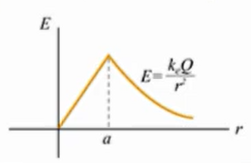
\includegraphics[width=0.3\textwidth]{8.4.I.1.PNG}
\end{center}

In this, the peak is the surface of the insulator. 

When in equilibrium, the excess charge on a conductor lies on the surface of the conductor, 
making the electric field equal to zero inside. The electric field is perpendicular to the surface of the conductor.
\begin{center}
    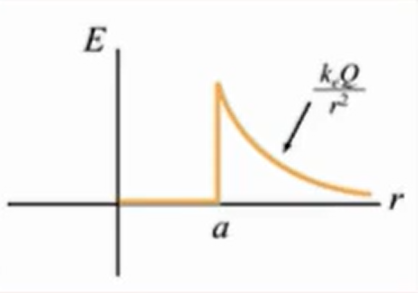
\includegraphics[width=0.3\textwidth]{8.4.I.2.PNG}
\end{center}

\begin{example}
    A particle of charge $2.0\times10^{-8}$C experiences an upward force of magnitude $4.0\times10^{-6}$N 
    when it is placed in a particular point in an electric field. 
    
    (a) What is the electric field at that point? 
    
    (b) If a charge $q=-1.0\times10^{-8}$C is placed there, what is the force on it?

    For part A:
    \[E=\frac{F_E}{q}=\frac{4.0\times10^{-6}\text{N}}{2.0\times10^{-8}\text{C}}=200\text{N/C upward}\]

    For part B:
    \[F_E=gE=(1.0\times10^{-8}\text{C})(200\text{N/C})=2.0\times10^{-6}\text{N downwards}\]
\end{example}


\section{Electric Fields of Charge Distributions}
The expressions for the electric field of specified charge distributions can be found using integration and the principle of superposition. 

Mathematically:
\[\vec{E}=\frac{1}{4\pi\epsilon_0}\int\frac{dq}{r^2}\hat{r}\]

Symmetry considerations of certain charge distributions can simplify analysis of the electric field resulting from those charge distributions.

Some common distributions are: Infinite Wire, Finite Wire, Semicircle (Arc), Ring of Charge 

There are three densities - linear, area, and volume. 

Linear: 
\[\lambda=\frac{Q}{L}\longrightarrow \lambda = \frac{dQ}{dL} \longrightarrow dQ=\lambda dL\]

Area: 
\[\sigma=\frac{Q}{A}\longrightarrow \sigma = \frac{dQ}{dA}\longrightarrow dQ=\sigma dA\]

Volume: 
\[\rho = \frac{Q}{V}\longrightarrow \rho = \frac{dQ}{dV} \longrightarrow DQ=\rho dV\]

At a point charge:
\[E_{PC}=\frac{kQ}{r^2} \therefore E=\frac{1}{4\pi\epsilon_0}\int \frac{dQ}{r^2}\hat{r}\]

\pagebreak
\begin{example}
    Derive an expression for the electric field at the center of a ring of charge with radius $a$ a distance $P$ away from the center.
    \begin{center}
        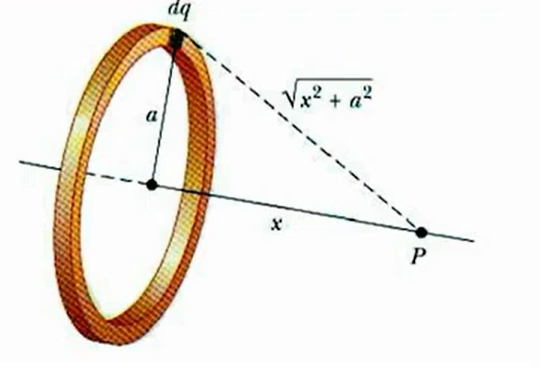
\includegraphics[width=0.3\textwidth]{8.5.PNG}
    \end{center}
    Note that $\sqrt{x^2+a^2}$, $a$, and $x$ are constant. 
    \smallbreak
    Looking at point $P$, there will be an infinite amount of electric fields caused by $dq$ at point $P$.
    \smallbreak
    All the y-components will cancel, so we will integrate through x.
    \begin{align*}
        E_{net}=dE_x=dE\cos\theta
        \\
        E_x=\frac{1}{4\pi\epsilon_0}\int\frac{dq}{r^2}
    \end{align*}
    We want to substitute $\frac{x}{\sqrt{x^2+a^2}}$ for $\cos\theta$.
    \begin{align*}
        E_x=\frac{1}{4\pi\epsilon_0}\int\frac{dq}{r^2}\cos\theta
        \\
        =\frac{1}{4\pi\epsilon_0}\int\frac{dq}{\sqrt{x^2+a^2}}\cdot\frac{x}{\sqrt{x^2+a^2}}
        \\
        =\frac{x}{4\pi\epsilon_0(x^2+a^2)^{3/2}}\int{dQ}
        \\
        =\frac{qx}{4\pi\epsilon_0(x^2+a^2)^{3/2}}
    \end{align*}
    This is the expression for the ring of charge. 
\end{example}

\ex Two charged rings are concentric and have radii $R$ and $2R$. Point $P$ is located on a line that passes through the common center of the rings and is perpendicular to the plane of the rings. Each ring is uniformly charged, initially with charges $+Q$ and $-Q$ on the ring of radius $2R$ and the ring of radius $R$, respectively. If each ring is given the opposite charge from what it had initially, what happens to the electric field magnitude $E$ at point $P$? What evidence or reasoning supports the claim?

\section{Electric Flux}
Flux describes the amount of a given quantity that passes through a given area.

For an electric field that is constant across an area, the electric flux through the area is defined as:
\[\phi_E=\vec{E}\cdot\vec{A}=EA\cos\theta\]
The direction of the area vector is defined as perpendicular to the plane of the surface and outward from closed surface.

The sign of the flux is given by the dot product of the electric field vector and the area vector.

The total electric flux passing through a surface is defined by the surface integral of the electric field over the surface:
\[\phi_E=\int\vec{E}\cdot\mathrm{d}\vec{A}=EA\]
\begin{example}
    A sphere of radius $r=2$ cm creates an electric field $E=3$N/C at a distance $d=5$ cm from the 
    center of the sphere. What is the electric flux through the surface of the sphere drawn at a distance $d=5$cm?
    \begin{center}
        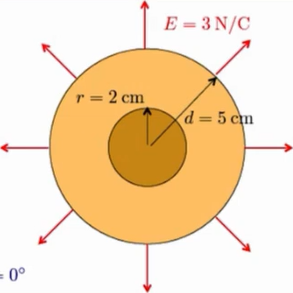
\includegraphics[width=0.3\textwidth]{8.6.PNG}
    \end{center}
    The surface area of a sphere is $4\pi r^2$, so
    \begin{align*}
        \phi_E=\int\vec{E}\cdot\mathrm{d}\vec{A}=EA=E(4\pi r^2)=(3)(4\pi(0.05)^2)=0.094\text{N}\cdot\text{m}^2\text{/C}
    \end{align*} 
\end{example}

\ex A positive point charge is located at the center of a sphere of variable radius $r$. Draw a graph that indicates the electric flux through the surface of the sphere as a function of its radius.

\section{Gauss's Law}
Gauss's law relates electric flux to a Gaussian surface to the charge enclosed by that surface:
\[\phi_E=\frac{q_{\text{enc}}}{\epsilon_0}=\oint\vec{E}\cdot\mathrm{d}\vec{A}=EA\]
A gaussian surface is a three-dimensional, closed surface. 

The total electric flux through the surface is independent of the size of the Gaussian 
surface if the amount of enclosed charge remains constant.

Surfaces are constructed such that the electric field generated by the enclosed 
charge is either perpendicular or parallel to different regions of the Gaussian surface.

If a function of charge density is given for a charge distribution, the total 
charge can be determined by integrating the charge density of the length (1D), area (2D), or volume (3D).

Maxwell's equations are the collection of equations that fully describe electromagnetism. The first of these is Gauss's Law.

\pagebreak
\begin{example}
    A spherical cloud of charge radius $R$ contains a total charge $+Q$ with a 
    nonuniform charge density that varies according to the equation:
    \begin{align*}
        \rho(r)=\rho_0\left(1-\frac{r}{R}\right) \text{ for } r\leq R \text{ and }\\
        \rho = 0 \text{ for } r>R\text{,}
    \end{align*}
    where $r$ is the distance from the center of the cloud. Express all algebraic answers in terms of $Q$, $R$, and fundamental constants. Determine the magnitude $E$ of the electric field when $r>R$.
    \begin{align*}
        \frac{q_\text{enc}}{\epsilon_0}=\int\vec{E}\cdot\mathrm{d}\vec{A}=EA=E(4\pi r^2)
        \\
        \implies E=\frac{1}{4\pi\epsilon_0}\cdot\frac{Q}{r^2}
    \end{align*}
\end{example}
\ex A solid insulating sphere of radius 10 cm has a net charge of 40 nC distributed uniformly throughout its volume. What is the electric field at a distance of 2.0 cm from the cneter of the sphere?

\ex A very long solid insulating cylinder of radius $R$ has a charge uniformly distributed over its volume, such that its overall linear charge is $\lambda$. What is the magnitude of the electric field at a perpendicular distance $r\leq R$ from the cylinder's central axis?

\section*{Review Questions}
\ex Three small charged spheres, $A$, $B$, and $C$, are placed along the $x$-axis at the positions shown in the figure. Spheres $A$ and $B$ have the same charge $Q$, while sphere $C$ has an unknown charge. 
\begin{center}
    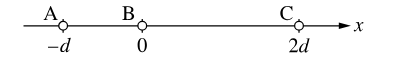
\includegraphics[width=0.5\textwidth]{8.1.AP.PNG}
\end{center}
If the net electrostatic force on sphere $B$ due to spheres $A$ and $C$ is zero, what is the magnitude of the net electrostatic force on Sphere $A$ due to spheres $B$ and $C$?

\ex A netural metal sphere is on an insulated stand. A charged rod then touches the sphere briefly, after which it is found that the metal sphere has a charge of 40 nC. 

Approximately how many electrons were transferred between the rod and the sphere?

\ex \begin{center}
    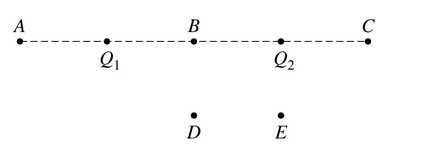
\includegraphics[width=0.5\textwidth]{8.3.AP.PNG}
\end{center}
Two point charges, $Q_1=+3\mu$C and $Q_2=-3\mu$C, are situated as shown in the figure above. 

At what labeled point is the magnitude of the electric field the greatest?

\pagebreak
\ex \begin{center}
    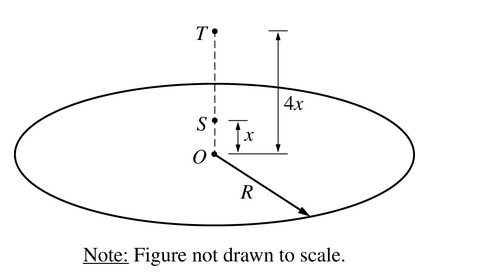
\includegraphics[width=0.5\textwidth]{8.4.AP.PNG}
\end{center}
The figure above shows a thin, circular nonconducting sheet of positive charge uniformly distributed over its area. The radius of the sheet is $R$. Point $O$ is at the center of the sheet.
Point $S$ is a distance $x$ from the center of the sheet, and point $T$ is a distance $4x$ from the center of the sheet. Assume $R>>x$. 

If the magnitude of the electric field at point $T$ is $E_T$, what represents the magnitude of the electric field at point $S$?

\ex Charge is distributed uniformly throughout a long nonconducting cylinder of radius $R$. Draw a graph that best represents the magnitude of the resulting field $E$ as a function of $r$, the distance from the axis of the cylinder.


\end{document}